
\documentclass[a4paper,11pt]{article}
\usepackage[a4paper, margin=8em]{geometry}

% usa i pacchetti per la scrittura in italiano
\usepackage[french,italian]{babel}
\usepackage[T1]{fontenc}
\usepackage[utf8]{inputenc}
\frenchspacing 

% usa i pacchetti per la formattazione matematica
\usepackage{amsmath, amssymb, amsthm, amsfonts}

% usa altri pacchetti
\usepackage{gensymb}
\usepackage{hyperref}
\usepackage{standalone}

\usepackage{colortbl}

\usepackage{xstring}
\usepackage{karnaugh-map}

% imposta il titolo
\title{Computer Architectures notes}
\author{Luca Seggiani}
\date{2026}

% imposta lo stile
% usa helvetica
\usepackage[scaled]{helvet}
% usa palatino
\usepackage{palatino}
% usa un font monospazio guardabile
\usepackage{lmodern}

\renewcommand{\rmdefault}{ppl}
\renewcommand{\sfdefault}{phv}
\renewcommand{\ttdefault}{lmtt}

% circuiti
\usepackage{circuitikz}
\usetikzlibrary{babel}

% testo cerchiato
\newcommand*\circled[1]{\tikz[baseline=(char.base)]{
            \node[shape=circle,draw,inner sep=2pt] (char) {#1};}}

% disponi il titolo
\makeatletter
\renewcommand{\maketitle} {
	\begin{center} 
		\begin{minipage}[t]{.8\textwidth}
			\textsf{\huge\bfseries \@title} 
		\end{minipage}%
		\begin{minipage}[t]{.2\textwidth}
			\raggedleft \vspace{-1.65em}
			\textsf{\small \@author} \vfill
			\textsf{\small \@date}
		\end{minipage}
		\par
	\end{center}

	\thispagestyle{empty}
	\pagestyle{fancy}
}
\makeatother

% disponi teoremi
\usepackage{tcolorbox}
\newtcolorbox[auto counter, number within=section]{theorem}[2][]{%
	colback=blue!10, 
	colframe=blue!40!black, 
	sharp corners=northwest,
	fonttitle=\sffamily\bfseries, 
	title=Theorem~\thetcbcounter: #2, 
	#1
}

% disponi definizioni
\newtcolorbox[auto counter, number within=section]{definition}[2][]{%
	colback=red!10,
	colframe=red!40!black,
	sharp corners=northwest,
	fonttitle=\sffamily\bfseries,
	title=Definition~\thetcbcounter: #2,
	#1
}

% disponi codice
\usepackage{listings}
\usepackage[table]{xcolor}

\definecolor{codegreen}{rgb}{0,0.6,0}
\definecolor{codegray}{rgb}{0.5,0.5,0.5}
\definecolor{codepurple}{rgb}{0.58,0,0.82}
\definecolor{backcolour}{rgb}{0.95,0.95,0.92}

\lstdefinestyle{codestyle}{
		backgroundcolor=\color{black!5}, 
		commentstyle=\color{codegreen},
		keywordstyle=\bfseries\color{magenta},
		numberstyle=\sffamily\tiny\color{black!60},
		stringstyle=\color{green!50!black},
		basicstyle=\ttfamily\footnotesize,
		breakatwhitespace=false,         
		breaklines=true,                 
		captionpos=b,                    
		keepspaces=true,                 
		numbers=left,                    
		numbersep=5pt,                  
		showspaces=false,                
		showstringspaces=false,
		showtabs=false,                  
		tabsize=2
}

\lstdefinestyle{shellstyle}{
		backgroundcolor=\color{black!5}, 
		basicstyle=\ttfamily\footnotesize\color{black}, 
		commentstyle=\color{black}, 
		keywordstyle=\color{black},
		numberstyle=\color{black!5},
		stringstyle=\color{black}, 
		showspaces=false,
		showstringspaces=false, 
		showtabs=false, 
		tabsize=2, 
		numbers=none, 
		breaklines=true
}

\lstdefinelanguage{x86}{ 
  keywords={AAA, AAD, AAM, AAS, ADC, ADCB, ADCW, ADCL, ADD, ADDB, ADDW, ADDL, AND, ANDB, ANDW, ANDL,
        ARPL, BOUND, BSF, BSFL, BSFW, BSR, BSRL, BSRW, BSWAP, BT, BTC, BTCB, BTCW, BTCL, BTR, 
        BTRB, BTRW, BTRL, BTS, BTSB, BTSW, BTSL, CALL, CBW, CDQ, CLC, CLD, CLI, CLTS, CMC, CMP,
        CMPB, CMPW, CMPL, CMPS, CMPSB, CMPSD, CMPSW, CMPXCHG, CMPXCHGB, CMPXCHGW, CMPXCHGL,
        CMPXCHG8B, CPUID, CWDE, DAA, DAS, DEC, DECB, DECW, DECL, DIV, DIVB, DIVW, DIVL, ENTER,
        HLT, IDIV, IDIVB, IDIVW, IDIVL, IMUL, IMULB, IMULW, IMULL, IN, INB, INW, INL, INC, INCB,
        INCW, INCL, INS, INSB, INSD, INSW, INT, INT3, INTO, INVD, INVLPG, IRET, IRETD, JA, JAE,
        JB, JBE, JC, JCXZ, JE, JECXZ, JG, JGE, JL, JLE, JMP, JNA, JNAE, JNB, JNBE, JNC, JNE, JNG,
        JNGE, JNL, JNLE, JNO, JNP, JNS, JNZ, JO, JP, JPE, JPO, JS, JZ, LAHF, LAR, LCALL, LDS,
        LEA, LEAVE, LES, LFS, LGDT, LGS, LIDT, LMSW, LOCK, LODSB, LODSD, LODSW, LOOP, LOOPE,
        LOOPNE, LSL, LSS, LTR, MOV, MOVB, MOVW, MOVL, MOVSB, MOVSD, MOVSW, MOVSX, MOVSXB,
        MOVSXW, MOVSXL, MOVZX, MOVZXB, MOVZXW, MOVZXL, MUL, MULB, MULW, MULL, NEG, NEGB, NEGW,
        NEGL, NOP, NOT, NOTB, NOTW, NOTL, OR, ORB, ORW, ORL, OUT, OUTB, OUTW, OUTL, OUTSB, OUTSD,
        OUTSW, POP, POPL, POPW, POPB, POPA, POPAD, POPF, POPFD, PUSH, PUSHL, PUSHW, PUSHB, PUSHA, 
        RCLL, RCR, RCRB, RCRW, RCRL, RDMSR, RDPMC, RDTSC, REP, REPE, REPNE, RET, ROL, ROLB, ROLW,
        ROLL, ROR, RORB, RORW, RORL, SAHF, SAL, SALB, SALW, SALL, SAR, SARB, SARW, SARL, SBB,
        SBBB, SBBW, SBBL, SCASB, SCASD, SCASW, SETA, SETAE, SETB, SETBE, SETC, SETE, SETG, SETGE,
        SETL, SETLE, SETNA, SETNAE, SETNB, SETNBE, SETNC, SETNE, SETNG, SETNGE, SETNL, SETNLE,
        SETNO, SETNP, SETNS, SETNZ, SETO, SETP, SETPE, SETPO, SETS, SETZ, SGDT, SHL, SHLB, SHLW,
        SHLL, SHLD, SHR, SHRB, SHRW, SHRL, SHRD, SIDT, SLDT, SMSW, STC, STD, STI, STOSB, STOSD,
        STOSW, STR, SUB, SUBB, SUBW, SUBL, TEST, TESTB, TESTW, TESTL, VERR, VERW, WAIT, WBINVD,
        XADD, XADDB, XADDW, XADDL, XCHG, XCHGB, XCHGW, XCHGL, XLAT, XLATB, XOR, XORB, XORW, XORL},
  keywordstyle=\color{blue}\bfseries,
  ndkeywordstyle=\color{darkgray}\bfseries,
  identifierstyle=\color{black},
  sensitive=false,
  comment=[l]{\#},
  morecomment=[s]{/*}{*/},
  commentstyle=\color{purple}\ttfamily,
  stringstyle=\color{red}\ttfamily,
  morestring=[b]',
  morestring=[b]"
}

\lstdefinelanguage{riscv}{
  keywords={
    LUI, AUIPC,
    JAL, JALR,
    BEQ, BNE, BLT, BGE, BLTU, BGEU,
    LB, LH, LW, LBU, LHU, LD,
    SB, SH, SW, SD,
    ADDI, SLTI, SLTIU, XORI, ORI, ANDI,
    SLLI, SRLI, SRAI,
    ADD, SUB, SLL, SLT, SLTU, XOR, SRL, SRA, OR, AND,
    ADDIW, SLLIW, SRLIW, SRAIW,
    ADDW, SUBW, SLLW, SRLW, SRAW,
    MUL, MULH, MULHSU, MULHU, DIV, DIVU, REM, REMU,
    MULW, DIVW, DIVUW, REMW, REMUW,
    LR.W, SC.W, AMOSWAP.W, AMOADD.W, AMOXOR.W,
    AMOAND.W, AMOOR.W, AMOMIN.W, AMOMAX.W,
    AMOMINU.W, AMOMAXU.W,
    LR.D, SC.D, AMOSWAP.D, AMOADD.D, AMOXOR.D,
    AMOAND.D, AMOOR.D, AMOMIN.D, AMOMAX.D,
    AMOMINU.D, AMOMAXU.D,
    FLW, FSW,
    FMADD.S, FMSUB.S, FNMSUB.S, FNMADD.S,
    FADD.S, FSUB.S, FMUL.S, FDIV.S, FSQRT.S,
    FSGNJ.S, FSGNJN.S, FSGNJX.S,
    FMIN.S, FMAX.S,
    FCVT.W.S, FCVT.WU.S, FCVT.S.W, FCVT.S.WU,
    FMV.X.W, FMV.W.X,
    FEQ.S, FLT.S, FLE.S,
    FLD, FSD,
    FMADD.D, FMSUB.D, FNMSUB.D, FNMADD.D,
    FADD.D, FSUB.D, FMUL.D, FDIV.D, FSQRT.D,
    FSGNJ.D, FSGNJN.D, FSGNJX.D,
    FMIN.D, FMAX.D,
    FCVT.W.D, FCVT.WU.D, FCVT.D.W, FCVT.D.WU,
    FCVT.S.D, FCVT.D.S,
    FMV.X.D, FMV.D.X,
    FEQ.D, FLT.D, FLE.D,
    CSRRW, CSRRS, CSRRC,
    CSRRWI, CSRRSI, CSRRCI,
    FENCE.I,
    FENCE,
    ECALL, EBREAK,
    MRET, SRET, URET,
    WFI,
    SFENCE.VMA,
    NOP, LI, LA, MV,
    NOT, NEG, NEGW,
    SEQZ, SNEZ, SLTZ, SGTZ,
    BEQZ, BNEZ, BLEZ, BGEZ, BLTZ, BGTZ,
    BGT, BLE, BGTU, BLEU,
    J, JR, RET,
    CALL, TAIL,
    RDINSTRET, RDCYCLE, RDTIME,
    CSRR, CSRW, CSRS, CSRC,
    CSRWI, CSRSI, CSRCI
  },
  keywordstyle=\color{blue}\bfseries,
  ndkeywordstyle=\color{darkgray}\bfseries,
  identifierstyle=\color{black},
  sensitive=false,
  comment=[l]{\#},
  morecomment=[s]{/*}{*/},
  commentstyle=\color{purple}\ttfamily,
  stringstyle=\color{red}\ttfamily,
  morestring=[b]',
  morestring=[b]"
}

\lstdefinelanguage{arm}{
  keywords={
    ADC, ADD, AND, BIC, CMN, CMP, EOR, MOV, MVN,
    RSB, RSC, SBC, SUB, TST, TEQ,
    MLA, MLS, MUL, SMLAL, SMULL, UMLAL, UMULL,
    QADD, QSUB, QDADD, QDSUB,
    QADD16, QADD8, QASX, QSAX,
    QSUB16, QSUB8, QSAX, QSUBADDX,
    ASR, LSL, LSR, ROR, RRX,
    B, BL, BX, BLX,
    BXJ,
    BEQ, BNE, BCS, BHS, BCC, BLO,
    BMI, BPL, BVS, BVC,
    BHI, BLS, BGE, BLT, BGT, BLE,
    BAL,
    LDR, LDRB, LDRH, LDRSB, LDRSH,
    LDRD, LDM, LDMIA, LDMIB, LDMDA, LDMDB,
    LDRT, LDRBT, LDRHT, LDRSBT, LDRSHT,
    STR, STRB, STRH, STRD,
    STM, STMIA, STMIB, STMDA, STMDB,
    STRT, STRBT, STRHT,
    PUSH, POP,
    SWP, SWPB,
    REV, REV16, REVSH,
    BFC, BFI, BFXIL, SBFX, UBFX,
    CLZ,
    LDREX, LDREXB, LDREXH, LDREXD,
    STREX, STREXB, STREXH, STREXD,
    DMB, DSB, ISB,
    MCR, MCRR, MRC, MRRC,
    MRS, MSR,
    CPS, SETEND, SVC, BKPT,
    CLREX, WFE, WFI, SEV,
    YIELD, NOP,
    VLDR, VSTR,
    VMOV, VABS, VNEG,
    VADD, VSUB, VMUL, VDIV,
    VMLA, VMLS, VNMLA, VNMLS, VNMUL,
    VMAX, VMIN,
    VSQRT,
    VCMP, VCMPE,
    VCVT,
    VCLZ, VCLS,
    VAND, VORR, VEOR, VBIC, VMVN,
    VLD1, VLD2, VLD3, VLD4,
    VST1, VST2, VST3, VST4,
    ADR, ADCS, ADDS, SUBS, MOVS, ANDS, ORRS, EORS
  },
  keywordstyle=\color{blue}\bfseries,
  ndkeywordstyle=\color{darkgray}\bfseries,
  identifierstyle=\color{black},
  sensitive=false,
  comment=[l]{@},
  morecomment=[l]{;},
  morecomment=[s]{/*}{*/},
  commentstyle=\color{purple}\ttfamily,
  stringstyle=\color{red}\ttfamily,
  morestring=[b]',
  morestring=[b]"
}

\lstset{style=codestyle, language=C}

% disponi sezioni
\usepackage{titlesec}

\titleformat{\section}
	{\sffamily\Large\bfseries} 
	{\thesection}{1em}{} 
\titleformat{\subsection}
	{\sffamily\large\bfseries}   
	{\thesubsection}{1em}{} 
\titleformat{\subsubsection}
	{\sffamily\normalsize\bfseries} 
	{\thesubsubsection}{1em}{}

% tikz
\usepackage{tikz}

% float
\usepackage{float}

% grafici
\usepackage{pgfplots}
\pgfplotsset{width=10cm,compat=1.9}

% disponi alberi
\usepackage{forest}

\forestset{
	rectstyle/.style={
		for tree={rectangle,draw,font=\large\sffamily}
	},
	roundstyle/.style={
		for tree={circle,draw,font=\large}
	}
}

% disponi algoritmi
\usepackage{algorithm}
\usepackage{algorithmic}
\makeatletter
\renewcommand{\ALG@name}{Algorithm}
\makeatother

% disponi numeri di pagina
\usepackage{fancyhdr}
\fancyhf{} 
\fancyfoot[L]{\sffamily{\thepage}}

\makeatletter
\fancyhead[L]{\raisebox{1ex}[0pt][0pt]{\sffamily{\@title \ \@date}}} 
\fancyhead[R]{\raisebox{1ex}[0pt][0pt]{\sffamily{\@author}}}
\makeatother

\begin{document}
% sezione (data)
\section{Lesson 20-10-26}

% stili pagina
\thispagestyle{empty}
\pagestyle{fancy}

% testo

In the last lesson we saw the structure of the Tomasulo architecture.
Now we look into the reservation stations and the register files in more details.

\subsubsection{Fields}

First off, the reservation station's records are made out of the following \textit{fields}:
\begin{center}
	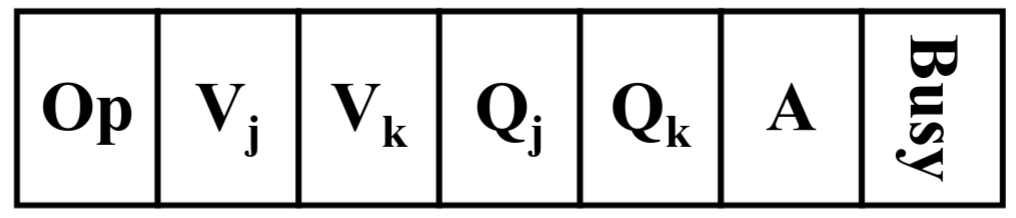
\includegraphics[scale=0.16]{../figures/res_stat_field.png}
\end{center}

These are:
\begin{itemize}
	\item $O_p$: represents the operation being performed on operands;
	\item $Q_j$, $Q_k$: the reservation station that will produce the relevant source operand (0 indicates the value is in $V_j$, $V_k$);
	\item $V_j$, $V_k$: the value of the source operands;
	\item $A$: used to hold the memory address information for a load or store;
	\item Busy: 1 if occupied, 0 if not occupied.
\end{itemize}

Information about which register is where is contained within the register file (floating point or integer): we store a $Q_i$ flag, which records the reservation station whose result should be stored in this register (if blank or 0, no values are destined for this register).

\subsubsection{Loads and stores}

Load and store instructions can be executed in
any order, provided that they do not refer to the
same address.
In this case, by exchanging their order:
\begin{itemize}
\item If the load is before the store, a WAR hazard
may happen;
\item If the store is before the load, a RAW hazard
may happen.
\end{itemize}

To avoid hazards coming from reordering load
and store instructions, the processor must:
\begin{itemize}
\item Compute memory addresses in order;
\item Perform some check for every load or store
instruction already in the buffers.
\end{itemize}

More formally:
\begin{itemize}
	\item When a \textbf{load} is about to be issued, the store buffer is checked for store
instructions acting on the same address, and the load is not issued until these previous instructions complete;
	\item When a \textbf{store} is about to be issued, both the load and store buffers are checked for load and store 
instructions acting on the same address, and the load is not issued until these previous instructions complete;
\end{itemize}

\subsection{Speculation}

This section follows pretty naturally from what we've seen so far:
\begin{itemize}
	\item First off we introduced the bare, unpipelined, processor;
	\item Then we introduced the \textit{pipeline}, and saw that hazards appear;
	\item When more than one execution unit was needed, we issued to pipelined stages via an issue unit in the \textit{Tomasulo architecture}. This showed that hazards were really dependencies showing up has hardware constraints.
\end{itemize}

We know extend the Tomasulo architecture by introducing \textbf{speculation}.

So far, when we met a branch instruction in the Tomasulo architecture, we stopped issuing instruction until the branch was taken.
We saw that when pipelining some kind of speculation could have been done on the branch outcome.
Let's see if we can do the same here.

Hardware-based speculation is a technique for
reducing the effects of control dependences in a
processor implementing dynamic scheduling.
If a processor supports branch prediction with
dynamic scheduling, it fetches and issues
instructions, as if the branch prediction was
always correct.
If a processor also supports hardware-based
speculation, it also \textit{executes} them.

It combines three ideas:
\begin{itemize}
	\item \textbf{Dynamic branch prediction}: we assume the result of branch instructions before they finish executing;
	\item \textbf{Dynamic scheduling}: we schedule instructions when they are \textit{ready} to execute;
	\item \textbf{Speculation}: we start executing the predicted instructions before the branch finishes executing..
\end{itemize}
In such a way, the processor implements \textbf{data
flow execution}: operations execute as soon as
their operands are available.

The basic Tomasulo’s architecture is adopted, extending
it to support speculation.
There are two different steps in instruction execution:
\begin{itemize}
\item The computation of results and their bypassing to
other instructions;
\item The update of register file and memory, which is only
performed when the instruction is no longer
speculative (\textit{instruction commit} via the \textbf{ROB} (\textit{ReOrder Buffer})); in this way, in-order commitment is implemented.
\end{itemize}

The ROB provides additional virtual registers and integrates the
store buffer existing in the original Tomasulo’s
architecture.

\begin{center}
	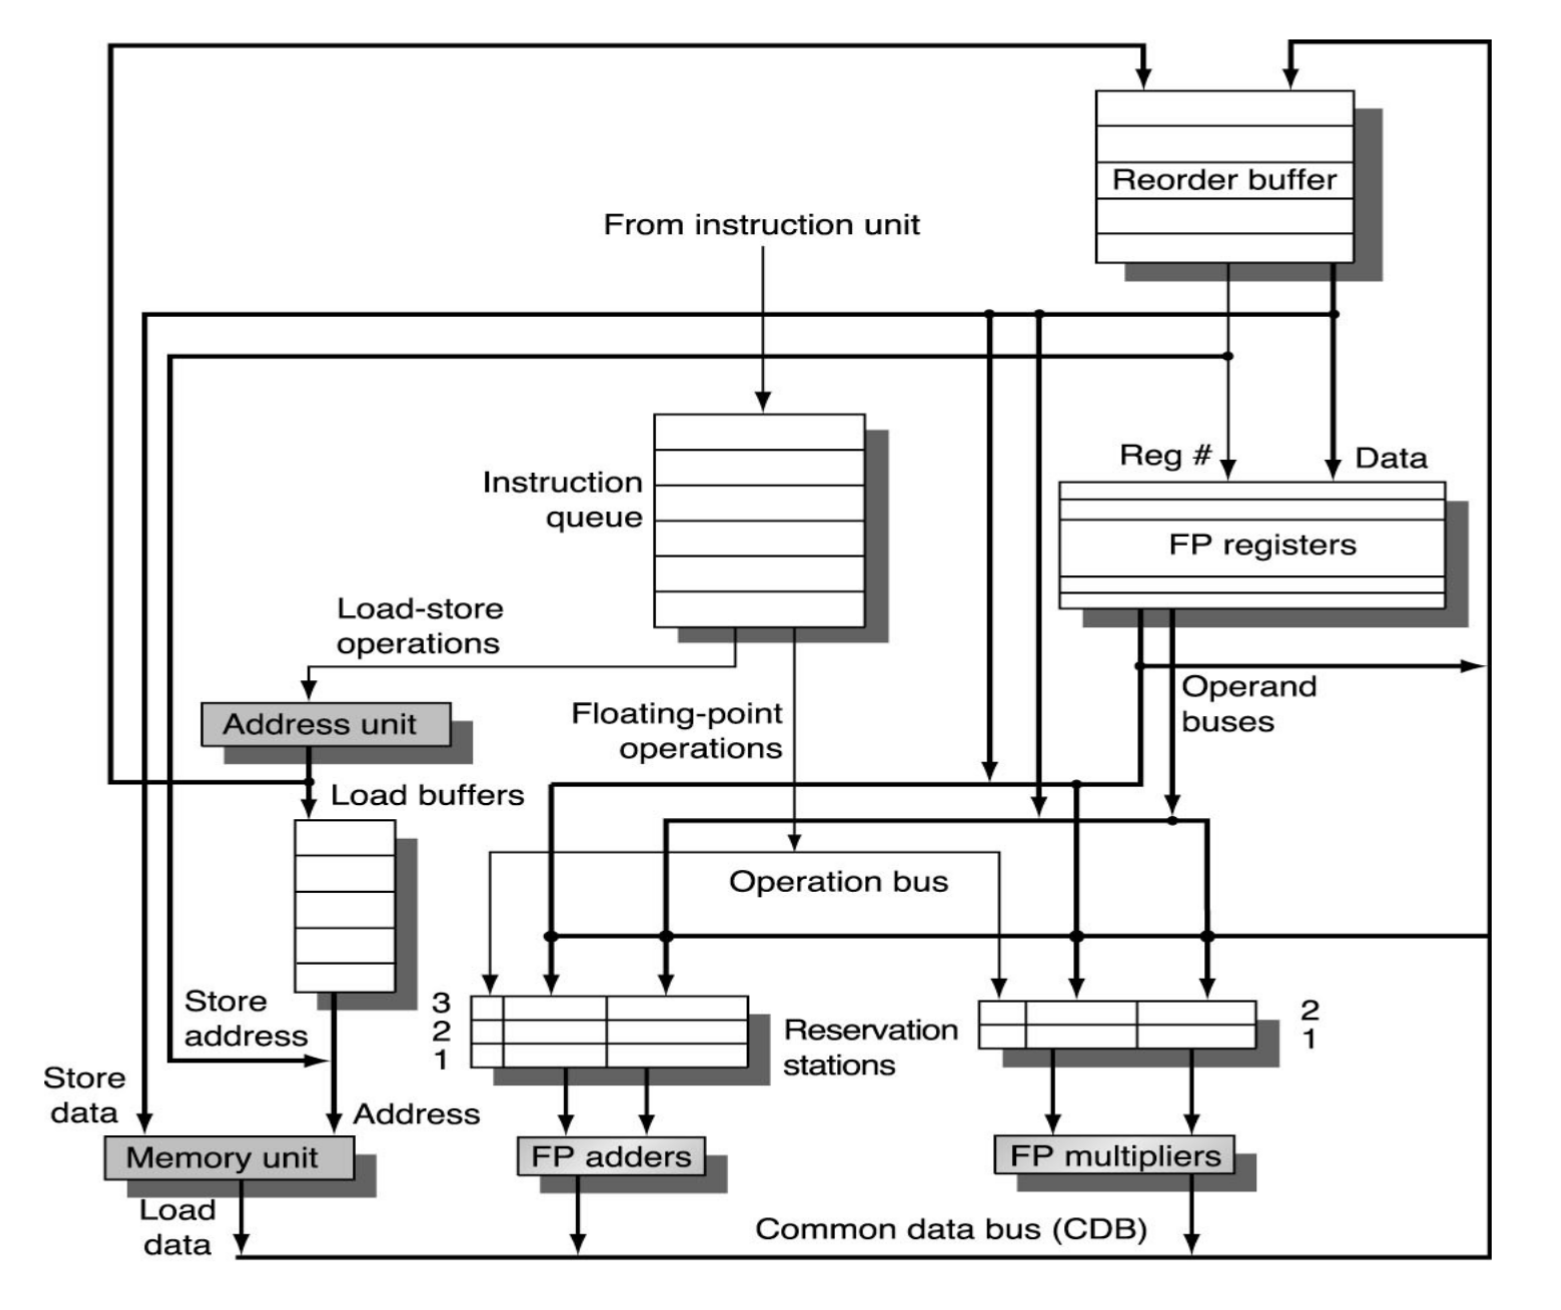
\includegraphics[scale=0.18]{../figures/rob.png}
\end{center}

\subsubsection{Fields}

Each ROB record has 4 \textit{fields}:
\begin{itemize}
\item Instruction type: branch, store, or register;
\item Destination: register number, or memory address;
\item Value: contains the value when the instruction has completed but still didn't commit to a register file;
\item Ready: indicates whether the instruction completed its execution.
\end{itemize}

With speculation, data for an incoming instruction may be read:
\begin{itemize}
	\item From the ROB, if the producing instruction didn't commit yet (because a branch wasn't confirmed);
	\item From the register file, otherwise (this is the normal execution path we saw this far).
\end{itemize}

\subsubsection{How does it work?}

An instruction is extracted from the instruction queue (that is, \textbf{issued}) if
there is:
\begin{itemize}
	\item An empty reservation station;
	\item An empty slot in the reorder buffer.
\end{itemize}

If this is not the case, the instruction issue is stalled.
Otherwise:
\begin{itemize}
	\item 
The operands for the instruction are sent to the
reservation station, if they are in the register file or in the
reorder buffer.
\item 
The number of the reorder buffer entry for the instruction
is sent to the reservation station to tag the instruction
(and its results, when they will be written on the \textbf{CDB} (\textit{Common Data Bus})).
\end{itemize}

\par\smallskip

At this point we want to know when this instruction will be \textbf{executed}.
The instruction is executed as soon as all the
required operands are available: this avoids any RAW hazard.
Operands are possibly taken from the CDB as soon
as another instruction produces them.
The length of this step of course varies depending on the
instruction type (and thus the execution unit that gets the instruction).

\par\smallskip

Next it's time for \textbf{writeback}.
As soon as it is available, the result is put on the
CDB (together with the tag identifying the
instruction) and sent to the Reorder Buffer.
Any reservation station waiting for the result reads
it, and the reservation station entry is marked as available

\par\smallskip

Why does this ensure control hazards are avoided?
The Reorder Buffer is ordered according to instructions
original order.
As soon as one instruction reaches the head of the buffer;
\begin{itemize}
\item If it is a mispredicted branch, the buffer is flushed, and
the execution is restarted with the correct successor of
the instruction;
\item Otherwise, the result is written in the register file or in
memory (in case of a store);
\item In both cases, the Reorder Buffer entry is marked as free.
The Reorder Buffer is implemented as a circular buffer.
\end{itemize}

\par\smallskip

The result of this is:
\begin{itemize}
	\item \textbf{WAR} and \textbf{WAW} name dependencies don't result in hazards, since dynamic renaming is implemented and memory updating occurs in-order (i.e., when a store reaches the top of the ROB).

		Register renaming is implemented via the \textbf{RAT} (\textit{Register Alias Table}) which assigns a physical register to a logical one. The RAT is updated every time an instruction is committed to a register.

	\item \textbf{RAW} hazards in memory are prevented by:
\begin{itemize}
\item Enforcing the program order while computing the
effective address of a load / store; 
\item Preventing a load to initiate its second step if any
active ROB entry occupied by a store has a
Destination field matching the A field of the load.
\end{itemize}

\textit{RAW} hazards in registers are of course prevented by the Tomasulo architecture itself.
\end{itemize}

\end{document}
